
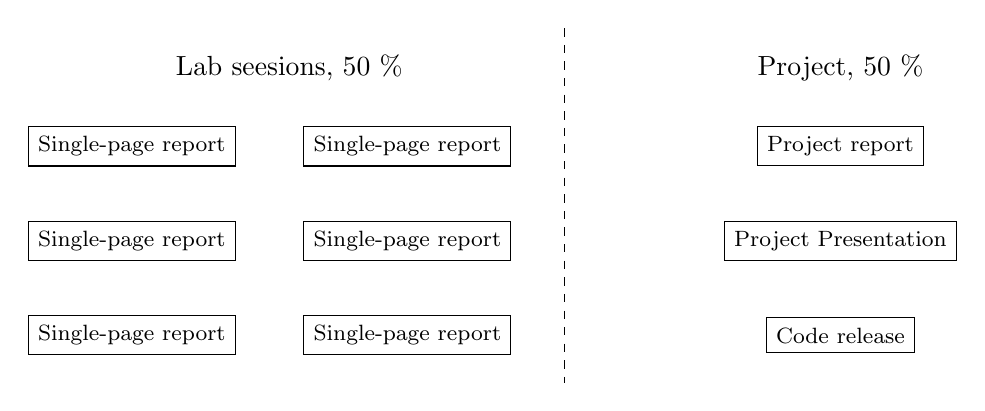
\begin{tikzpicture}[]

\foreach \i in {0,...,2} {
    \node[anchor=center, align=center, font=\footnotesize] (lr\i) at (-5.5, -1.2*\i) {Single-page report};
    \draw[black] (lr\i.south west) rectangle (lr\i.north east);
    
    \node[anchor=center, align=center, font=\footnotesize] (rr\i) at (-2, -1.2*\i) {Single-page report};
    \draw[black] (rr\i.south west) rectangle (rr\i.north east);
}

\node[anchor=center, align=center, font=\footnotesize] (pr) at (3.5,0) {Project report};
\draw[black] (pr.south west) rectangle (pr.north east);
    
\node[anchor=center, align=center, font=\footnotesize] (pp) at (3.5,-1.2) {Project Presentation};
\draw[black] (pp.south west) rectangle (pp.north east);
    
\node[anchor=center, align=center, font=\footnotesize] (cr) at (3.5,-2.4) {Code release};
\draw[black] (cr.south west) rectangle (cr.north east);


\draw[dashed] (0, 1.5) -- (0, -3);

\node[] at (-3.5, 1) {Lab seesions, 50 \%};
\node[] at ( 3.5, 1) {Project, 50 \%};


\end{tikzpicture}
